\chapter{Esperimenti e risultati}\label{chapter:implementazione}
Nel presente capitolo, verrà fornita un'esaustiva descrizione della metodologia impiegata nell'esperimento condotto per addestrare i diversi LLM utilizzando il framework QLoRA insieme al tool di Hugging Face denominato Autotrain Advanced. Tale metodologia ha consentito di configurare agevolmente i parametri di addestramento e, grazie all'infrastruttura di calcolo ad alte prestazioni dell'Ateneo (HPC), a schedulare diverse attività di addestramento per diverse epoche. Successivamente verranno presentate le valutazioni ed i risultati ottenuti durante gli esperimenti.



\section{Preparazione del dataset}\label{sec:dataset}

%linea logica di preparazione dataset:
%- la scelta del dataset
%- dove e` stato preso il dataset
%- l'elaborazione effettuata
%- aspettativa del progetto
%- esempi

Per questo esperimento è stata identificata una struttura di dati comune per poter addestrare gli LLM.
Il dataset è stato preso da \textbf{\href{https://scryfall.com/}{Scryfall}}, un database completo  di tutte le carte di \textit{Magic} che espone una serie di API con le quali è possibile ottenere l'intera collezione di carte organizzate sotto una struttura di un oggetto JSON simile a come descritta in Codice \ref{lst:input_example}.
Il dataset è stato elaborato\footnote{Notebook disponibile al repository \href{https://github.com/ZarakiKanzaki/project-lunar-ML/blob/main/ExploratoryDataAnalysisScryfall.ipynb}{ZarakiKanzaki/project-lunar-ML} su GitHub} utilizzando la libreria \textit{pandas}. È stata effettuata una pulitura delle proprietà che non fossero utili al fine di generare gli script (note legali, immagine, nome dell'artista, ecc.).
Una sfida relativa al dataset è stata quella di identificare i tipi di layout delle carte utilizzate in \emph{Magic}: durante i diversi anni di progettazione, i designer di \textit{Wizards of the Coast} hanno ideato diversi modi creativi di utilizzare le carte da gioco, alcune delle quali sopravvissute alle sfide del tempo. All'interno del dataset questo tipo di carte con diverse modalità di lettura (fronte-retro, carte split, carte ruotabili, ecc.) vengono rappresentate come una collezione di due carte, ovvero è presente una proprietà \textit{faces} che contiene le regole di ogni faccia della carta. Sebbene a livello di gioco possono esserci diverse regole per il tipo di layout, l'unico punto di interesse risiede nel dover descrivere gli effetti. Alcuni esempi di carte con layout diversi è presentato in figura \ref{fig:mfc}.
\begin{algorithm}[ht]
	\caption{Esempio di input da convertire}
	\label{lst:input_example}
	\begin{Verbatim}[numbers=left,breaklines]
{
    "name": "Primeval Titan",
    "mana_cost": "{4}{G}{G}",
    "type_line": "Creature \u2014 Giant",
    "oracle_text": "Trample\nWhenever Primeval Titan enters the battlefield or attacks, you may search your library for up to two land cards, put them onto the battlefield tapped, then shuffle.",
    "power": "6",
    "toughness": "6"
}
	\end{Verbatim}
\end{algorithm}

\begin{figure}[ht]
	\centering
	\begin{subfigure}{0.25\textwidth}
		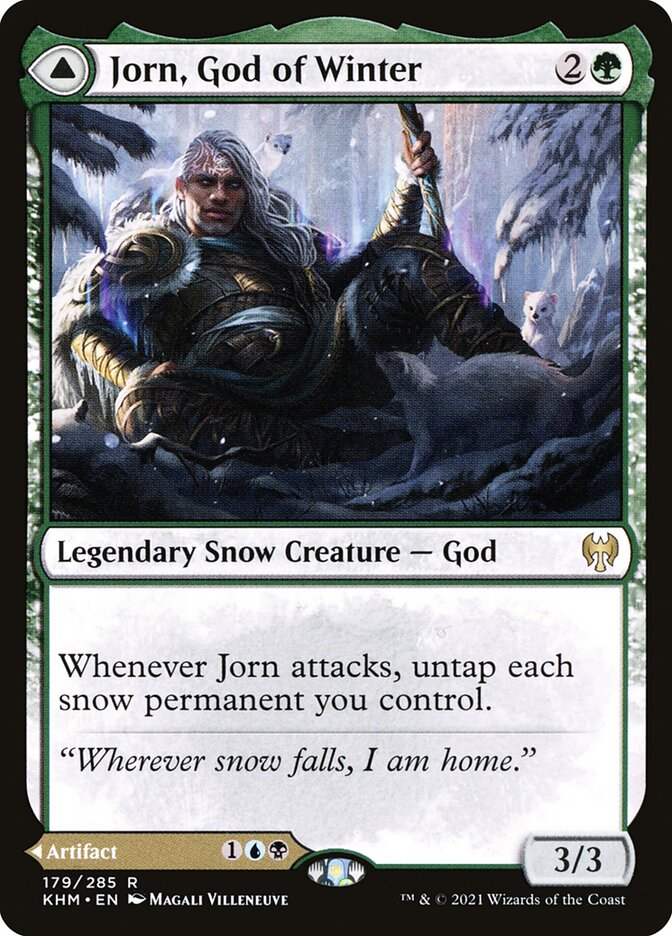
\includegraphics[width=1.0\textwidth]{Immagini/khm-179-jorn-god-of-winter.jpg}
	\end{subfigure}%
	\begin{subfigure}{0.25\textwidth}
		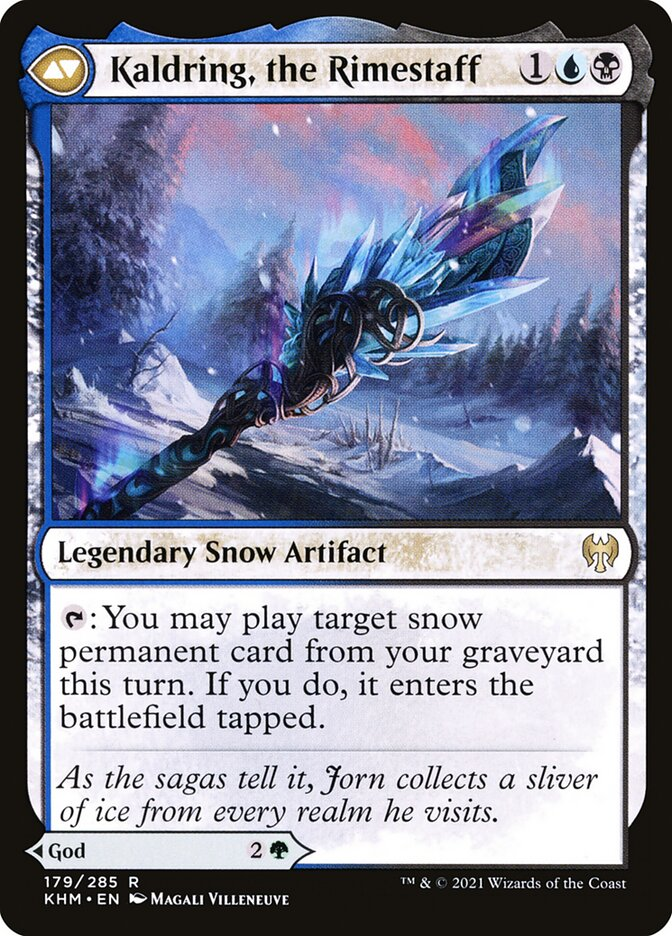
\includegraphics[width=1.0\textwidth]{Immagini/khm-179-kaldring-the-rimestaff.jpg}
	\end{subfigure}%
 	\begin{subfigure}{0.25\textwidth}
		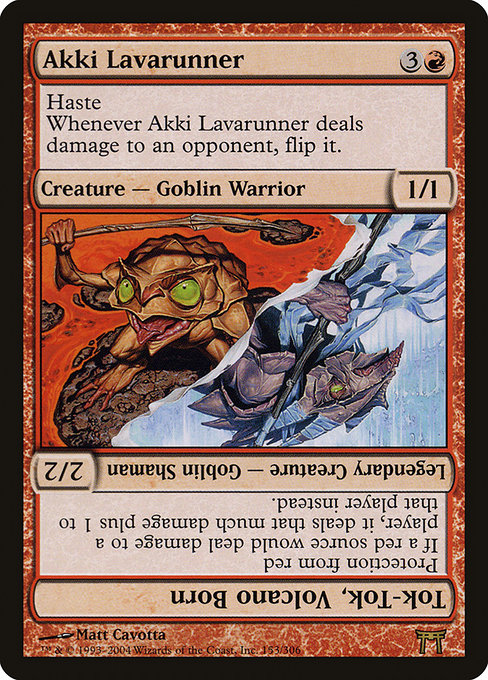
\includegraphics[width=1.0\textwidth]{Immagini/akki.jpg}
	\end{subfigure}%
 	\begin{subfigure}{0.25\textwidth}
		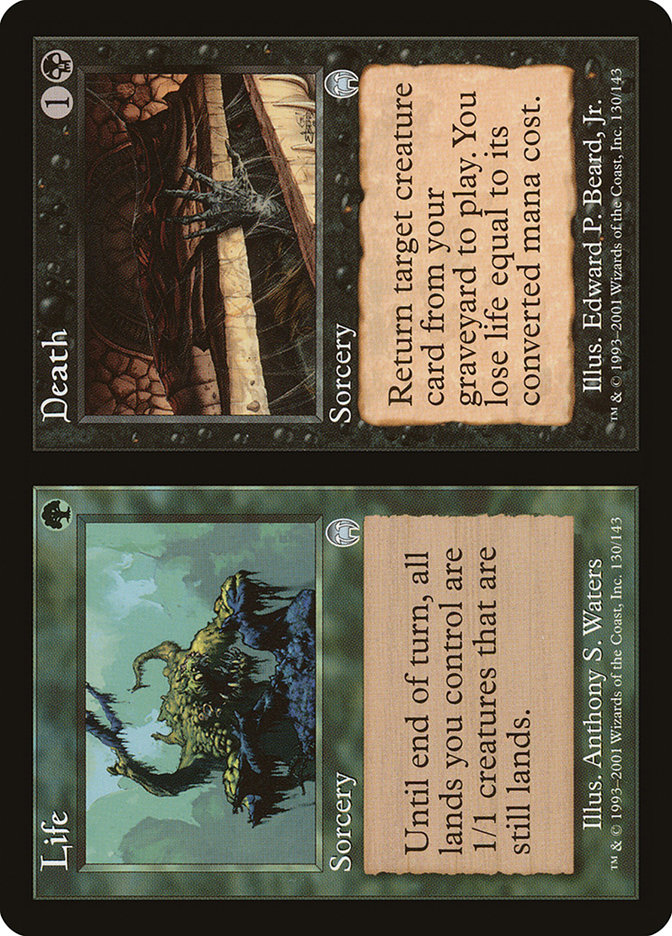
\includegraphics[width=1.0\textwidth]{Immagini/apc-130-life.jpg}
	\end{subfigure}
	\caption{Carte con layout differenti}
	\label{fig:mfc}
\end{figure}

Sono state analizzate circa 35.000 carte all'interno delle quali si possono identificare  20.000 effetti unici, alcuni sviluppatori hanno tentato di utilizzare una ResNet ottenendo un'accuratezza del 50\% \cite{forgescribe}.

Una volta effettuata questa esplorazione sui dati, è stato preparato un dataset\footnote{disponile al repository di HuggingFace \href{https://huggingface.co/datasets/404NotF0und/MtG-json-to-ForgeScript}{404NotF0und/MtG-json-to-ForgeScript}} per addestrare gli LLM, si è scelto di utilizzare un file \textit{csv} contenente 4 colonne: istrizione, input, risposta ed il campo testo, che  contiene il prompt utilizzato per l'addestramento. Di seguito è riportata la struttura di un singolo prompt per l'addestramento (Codice \ref{lst:train_prompt_structure}) ed un esempio di prompt nel Codice \ref{lst:train_prompt_example}.

\begin{algorithm}[ht]
	\caption{Struttura prompt per l'addestramento}
	\label{lst:train_prompt_structure}
	\begin{Verbatim}[numbers=left,breaklines]
Below is an instruction that describes a task then the input and response. 
### Instruction: Create the Forge script for this magic card 
### Input: <Il JSON della carta da generare>
### Response: <Lo script scritto in ForgeScript della carta> 
	\end{Verbatim}
\end{algorithm}

\begin{algorithm}[ht]
	\caption{Esempio di prompt per l'addestramento}
	\label{lst:train_prompt_example}
    \scriptsize
	\begin{Verbatim}[numbers=left,breaklines]
Below is an instruction that describes a task then the input and response. 
### Instruction: Create the Forge script for this magic card 
### Input: {"name": "Primeval Titan", "mana_cost": "{4}{G}{G}", "type_line": "Creature \u2014 Giant", "oracle_text": "Trample\nWhenever Primeval Titan enters the battlefield or attacks, you may search your library for up to two land cards, put them onto the battlefield tapped, then shuffle.", "power": "6", "toughness": "6"} 
### Response: Name:Primeval Titan\nManaCost:4 G G\nTypes:Creature Giant\nPT:6/6\nK:Trample\nT:Mode$ ChangesZone | Origin$ Any | Destination$ Battlefield | ValidCard$ Card.Self | Execute$ TrigChange | OptionalDecider$ You | TriggerDescription$ Whenever CARDNAME enters the battlefield or attacks, you may search your library for up to two land cards, put them onto the battlefield tapped, then shuffle.\nT:Mode$ Attacks | ValidCard$ Card.Self | Execute$ TrigChange | TriggerZones$ Battlefield | OptionalDecider$ You | Secondary$ True | TriggerDescription$ Whenever CARDNAME enters the battlefield or attacks, you may search your library for up to two land cards, put them onto the battlefield tapped, then shuffle.\nSVar:TrigChange:DB$ ChangeZone | Origin$ Library | Destination$ Battlefield | Tapped$ True | ChangeType$ Land | ChangeNum$ 2 | ShuffleNonMandatory$ True\nSVar:HasAttackEffect:TRUE\nOracle:Trample\nWhenever Primeval Titan enters the battlefield or attacks, you may search your library for up to two land cards, put them onto the battlefield tapped, then shuffle.
	\end{Verbatim}
\end{algorithm}


\section{Autotrain Advanced}\label{sec:autotrain_advanced}
AutoTrain di Hugging Face è uno strumento no-code per addestrare modelli all'avanguardia per compiti di Elaborazione del Linguaggio Naturale (NLP),  compiti di Computer Vision (CV), compiti tabellari e per compiti di elaborazione e generazione di Immagini.
Utilizzando AutoTrain Advanced, gli utenti avanzati possono controllare gli iperparametri utilizzati per l'addestramento di un qualsiasi modello, consentendo di addestrare più modelli con iperparametri diversi e confrontare i risultati.



\subsection{Addestramento}\label{sec:hpc_unipr_autotrain}

Inizialmente, si era pensato di utilizzare il servizio gratuito di Google Colab o Kaggle per l'addestramento, ma a causa delle limitazioni hardware e dei problemi legati al timeout delle versioni gratuite, si è deciso di richiedere l'accesso all'infrastruttura di calcolo ad alte prestazioni (High Performance Computing) dell'Ateneo.

Per gli esperimenti, si è scelto di utilizzare una GPU NVIDIA A100 da 80GB. L'addestramento è stato effettuato per diversi tagli di epoche, nello specifico 3, 10 e 20 epoche, al fine di arginare la limitazione delle 24 ore di utilizzo di una risorsa impostata dal HPC. I modelli di linguaggio utilizzati durante l'addestramento sono: Llama2-7B, OpenHermes-7B, TinyLlama, phi-2, Mistral-7B e Orca-2-13B.

Di seguito vengono spiegati i parametri del comando utilizzato per ogni addestramento, sia per il taglio di epoche che per gli LLM utilizzati, il comando è descritto dal Codice \ref{lst:autotrain-train}.\newline\newline

\begin{algorithm}[ht]
	\caption{Comando per l'addestramento con Autotrain Advanced}
	\label{lst:autotrain-train}
 \scriptsize
	\begin{Verbatim}[numbers=left,breaklines]
autotrain llm \
--train \
--model $LLM_FULLNAME \
--project-name lunar-llm-$LLM_NAME \
--data-path /MtG-json-to-ForgeScript/ \
--text-column text \
--lr 1e-4 \
--batch-size $BATCH_SIZE \
--epochs $EPOCHS \
--block-size 1024 \
--warmup-ratio 0.1 \
--lora-r 64 \
--lora-alpha 16 \
--lora-dropout 0.1 \
--weight-decay 0.01 \
--gradient-accumulation 4 \
--quantization int4 \
--mixed-precision fp16 \
--merge_adapter \
--peft\
--push-to-hub --token $HF_TOKEN \
--repo-id 404NotF0und/lunar-llm-$LLM_NAME
	\end{Verbatim}
\end{algorithm}
 
 I parametri utilizzati nel comando sono:

\begin{enumerate}[label=\alph*.]

  \item \texttt{--warmup-ratio 0.1}: Il rapporto di riscaldamento (warmup ratio) è utilizzato nell'ottimizzazione con un learning rate variabile. Durante le prime epoche dell'addestramento, il learning rate viene aumentato gradualmente fino a raggiungere il valore massimo. Il rapporto di riscaldamento indica la frazione di epoche totali utilizzate per il riscaldamento. In questo caso, il 10\% delle epoche totali viene utilizzato per il riscaldamento.
  
  \item \texttt{--lora-r 64}: Il parametro $r$ di LoRA (Layer-wise Relevance Propagation) indica il numero di vettori di rango basso che vengono utilizzati per approssimare i pesi del modello. Un valore più elevato di $r$ può migliorare l'accuratezza dell'approssimazione, ma aumenta anche la complessità computazionale. 
  
  \item \texttt{--lora-alpha 16}: Il parametro $\alpha$ di LoRA controlla il bilanciamento tra la sparsità e la precisione dell'approssimazione. Un valore più elevato di $\alpha$ favorisce la sparsità a scapito della precisione. 
  
  \item \texttt{--lora-dropout 0.1}: Il dropout di LoRA è una tecnica di regolarizzazione utilizzata per prevenire l'overfitting durante l'addestramento. Il dropout viene applicato ai vettori di rango basso in LoRA, e il parametro specifica la probabilità che un elemento venga azzerato. 
  
  \item \texttt{--weight-decay 0.01}: Il decadimento del peso (weight decay) è un altro metodo di regolarizzazione che aggiunge una penalità L2 alla funzione obiettivo. Il parametro controlla l'intensità della penalità: valori più alti corrispondono a una regolarizzazione più forte. 
  
  \item \texttt{--gradient-accumulation 4}: L'accumulo del gradiente è una tecnica utilizzata per ridurre la frequenza degli aggiornamenti del modello durante l'addestramento. Invece di aggiornare il modello ad ogni passo, i gradienti vengono accumulati per un certo numero di passi e poi aggiornati. Questo può migliorare la stabilità e la qualità dell'addestramento, specialmente quando si utilizzano batch di dimensioni ridotte. 
  
  \item \texttt{--quantization int4}: La quantizzazione è una tecnica utilizzata per ridurre la dimensione e la complessità computazionale del modello. In questo caso, la quantizzazione int4 implica che i pesi del modello vengono rappresentati con interi a 4 bit, riducendo così la dimensione del modello e accelerando l'inferenza.
  
  \item \texttt{--mixed-precision fp16}: La precisione mista si riferisce all'utilizzo di diversi tipi di dati per rappresentare i pesi, gli attivazioni e i gradienti durante l'addestramento. In questo caso, la precisione mista fp16 indica che i calcoli vengono eseguiti in parte con numeri in virgola mobile a 16 bit (half-precision) e in parte con numeri in virgola mobile a 32 bit (single-precision). Questo può accelerare l'addestramento e ridurre l'utilizzo di memoria senza compromettere significativamente l'accuratezza del modello.
\end{enumerate}




\subsection{Funzione obiettivo}\label{sec:loss_function}
Autrain Advanced utilizza come funzione obiettivo la \textit{cross Entropia}.
La cross entropia è una funzione di perdita comunemente utilizzata nell'addestramento degli LLM e di altri modelli di classificazione basati sull'apprendimento profondo. La cross entropia misura la differenza tra due distribuzioni di probabilità, in questo caso, la distribuzione di probabilità prevista dal modello e la distribuzione di probabilità vera dei dati. Durante l'addestramento, l'obiettivo è minimizzare la cross entropia, il che significa che si cerca di avvicinare il più possibile la distribuzione di probabilità prevista dal modello a quella dei dati reali.

Nel contesto degli LLM, la cross entropia viene utilizzata per misurare la differenza tra le probabilità delle parole previste dal modello e le parole effettivamente osservate nel testo di addestramento. Poiché gli LLM sono modelli generativi, durante l'addestramento cercano di prevedere la parola successiva in una sequenza di testo, data una sequenza di parole precedenti. La cross entropia viene utilizzata per quantificare la ``sorpresa" del modello rispetto alle parole osservate, penalizzando le previsioni errate e premiando quelle corrette.

La cross entropia \(H(p, q)\) tra due distribuzioni di probabilità \(p\) e \(q\) è definita come:

\[H(p, q) = -\sum_{i} p(i) \log q(i)\]

dove \(i\) indica un evento (ad esempio, una parola nel contesto degli LLM), \(p(i)\) è la probabilità dell'evento \(i\) secondo la distribuzione di probabilità vera \(p\), e \(q(i)\) è la probabilità dell'evento \(i\) secondo la distribuzione di probabilità prevista dal modello \(q\). Il logaritmo è tipicamente in base 2 o in base $e$ (logaritmo naturale).

Durante l'addestramento di un LLM, la cross entropia viene calcolata su tutto il testo di addestramento e viene utilizzata per aggiornare i parametri del modello tramite tecniche di ottimizzazione, come la discesa del gradiente. Poiché la cross entropia tiene conto delle probabilità di tutte le parole nel vocabolario, essa incoraggia il modello a generare previsioni accurate non solo per le parole comuni, ma anche per quelle meno frequenti, migliorando la capacità del modello di catturare la struttura e le sfumature del linguaggio naturale \cite{cross_entropy}.

In sintesi, la cross entropia è una funzione di perdita fondamentale nell'addestramento degli LLM, poiché misura la differenza tra le probabilità previste dal modello e le probabilità vere dei dati. Minimizzare la cross entropia durante l'addestramento permette al modello di apprendere rappresentazioni linguistiche accurate e coerenti, migliorando la sua capacità di comprendere e generare il linguaggio naturale.
\begin{figure}[ht]
	\centering
	\begin{subfigure}{0.33\textwidth}
		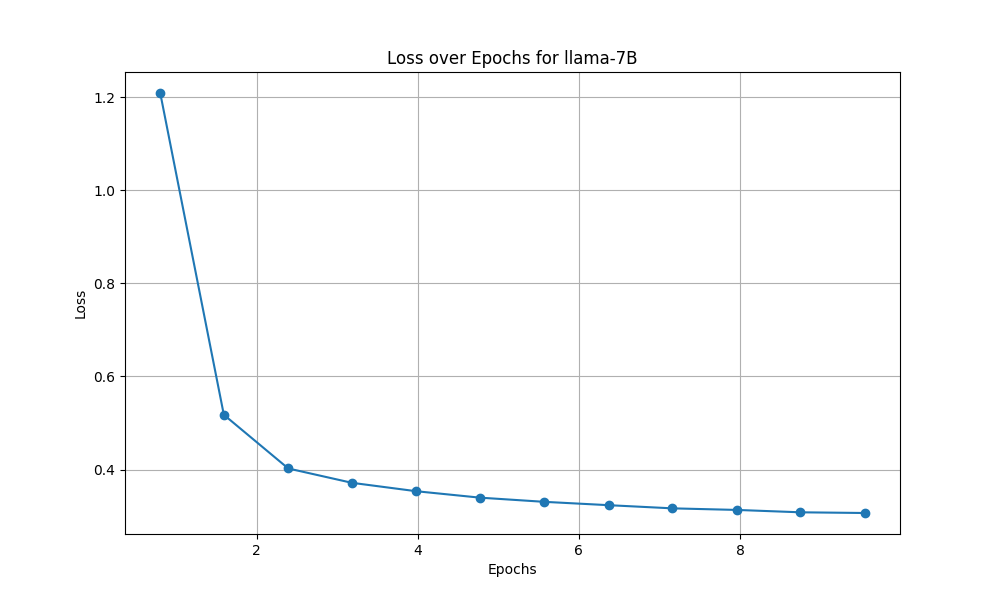
\includegraphics[width=1.0\textwidth]{Immagini/train_loss/llama-7B-loss_plot.png}
		\caption{Llama-7B}
	\end{subfigure}%
	\begin{subfigure}{0.33\textwidth}
		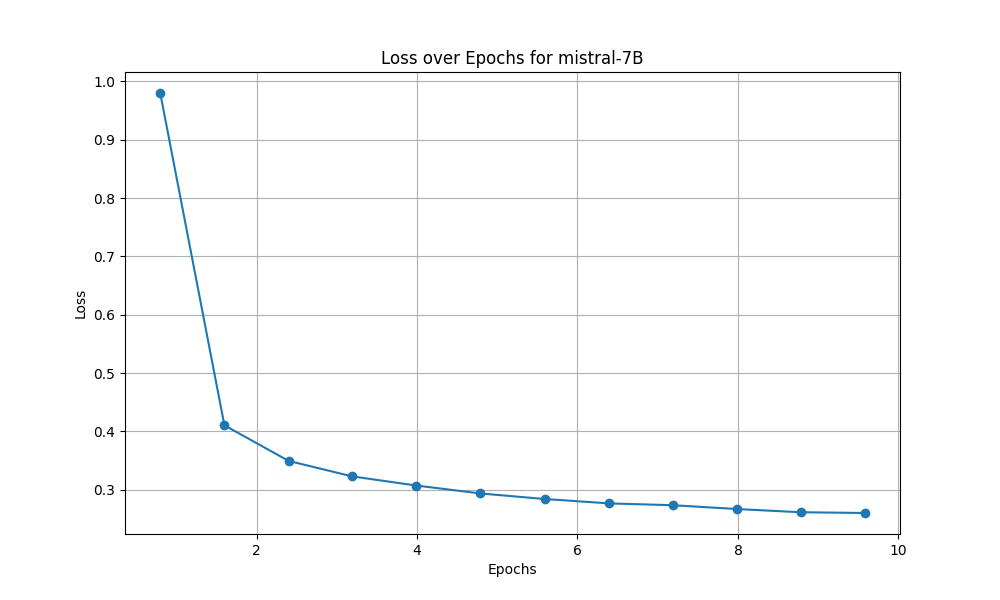
\includegraphics[width=1.0\textwidth]{Immagini/train_loss/mistral-7B-loss_plot.png}
		\caption{Mistral-7B}
	\end{subfigure}%
 	\begin{subfigure}{0.33\textwidth}
		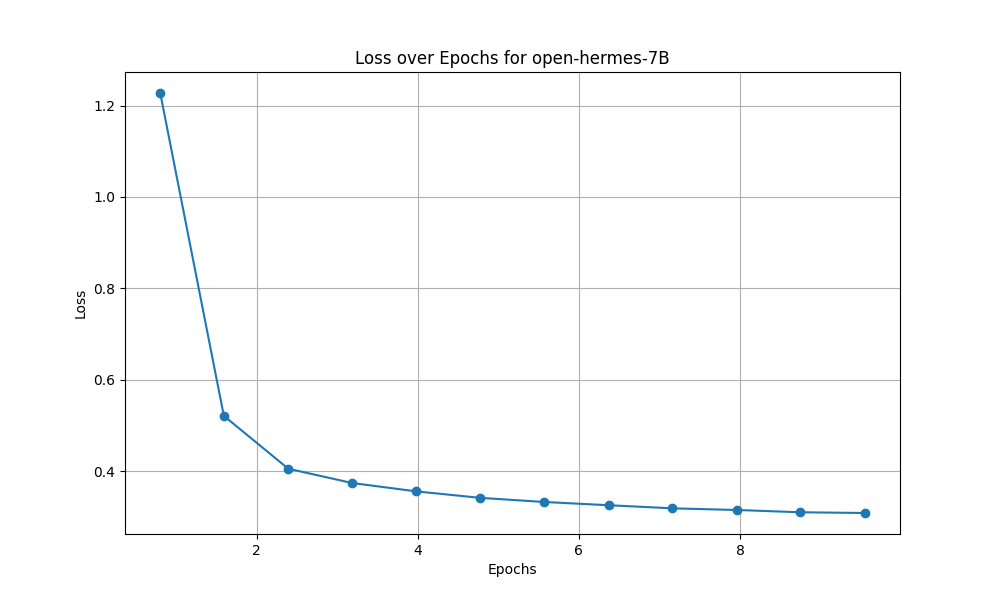
\includegraphics[width=1.0\textwidth]{Immagini/train_loss/open-hermes-7B-loss_plot.png}
		\caption{OpenHermes-7B}
	\end{subfigure}
  	\begin{subfigure}{0.33\textwidth}
		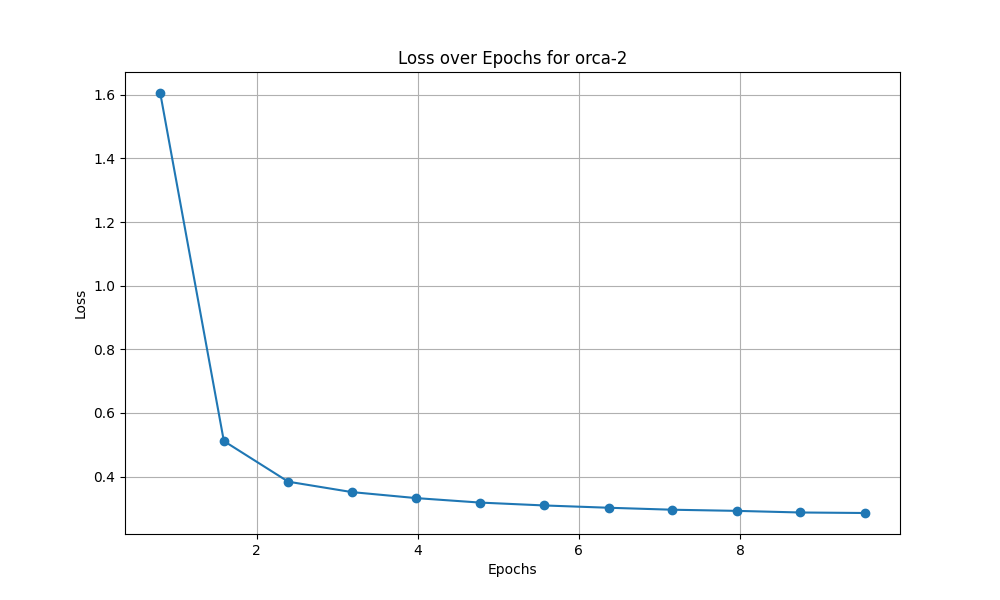
\includegraphics[width=1.0\textwidth]{Immagini/train_loss/orca-2-loss_plot.png}
		\caption{Orca-2}
	\end{subfigure}%
	\begin{subfigure}{0.33\textwidth}
		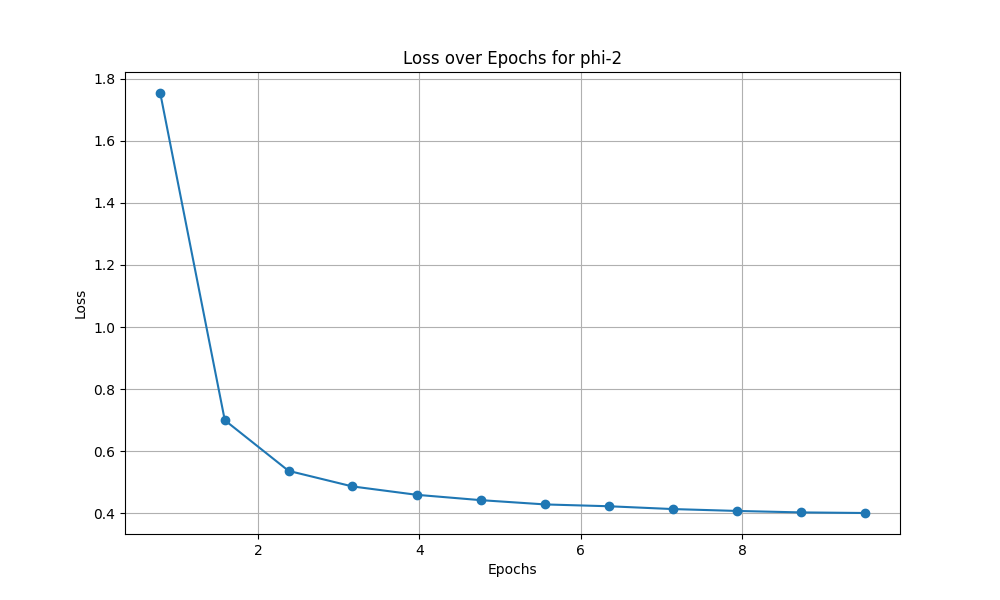
\includegraphics[width=1.0\textwidth]{Immagini/train_loss/phi-2-loss_plot.png}
		\caption{phi-2}
	\end{subfigure}%
 	\begin{subfigure}{0.33\textwidth}
		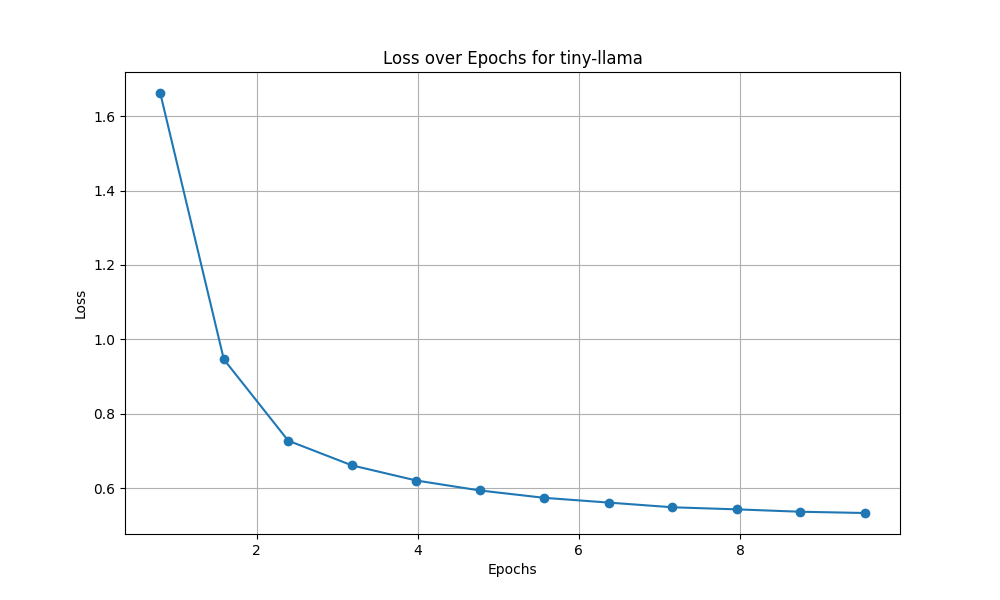
\includegraphics[width=1.0\textwidth]{Immagini/train_loss/tiny-llama-loss_plot.png}
		\caption{TinyLlama}
	\end{subfigure}
	\caption{Funzione di cross-Entropia per i vari llm}
	\label{fig:llm-loss_function}
\end{figure}



\subsection{Metriche di valutazione}\label{sec:hpc_unipr_evaluation_metrics}
Per prima cosa occorre identificare quali metriche utilizzate in questo esperimento:



\begin{enumerate}[label=\alph*.]

  \item \textbf{Perplexity}: La perplexity è una misura di quanto bene un modello di linguaggio probabilistico riesce a prevedere un campione di testo. Essa corrisponde all'inverso della radice n-esima della probabilità del prodotto assegnata al testo dal modello, dove n è il numero di parole nel testo. Un valore di perplexity più basso indica che il modello ha una maggiore probabilità di prevedere correttamente il testo e, in generale, un modello con una perplexity minore è considerato migliore. La formula per calcolare la perplexity è la seguente:

\[PP(W) = \sqrt[N]{\frac{1}{P(w_1,w_2,\dots,w_N)}}\]

dove $PP(W)$ è la perplexity, $P(w_1,w_2,\dots,w_N)$ è la probabilità del prodotto assegnata al testo dal modello e $N$ è il numero di parole nel testo.

  \item \textbf{Edit Distance}: L'edit distance, o distanza di Levenshtein, è una metrica che quantifica la differenza tra due stringhe di caratteri. Essa rappresenta il numero minimo di singole operazioni di modifica (inserimenti, eliminazioni o sostituzioni di caratteri) necessarie per trasformare una stringa nell'altra. Un valore di edit distance più basso indica che le due stringhe sono più simili tra loro. L'edit distance è spesso utilizzata per valutare la qualità delle traduzioni automatiche o delle correzioni ortografiche.

  \item \textbf{Accuracy}: L'accuracy è una metrica utilizzata per valutare la performance di un modello di classificazione. Essa rappresenta il rapporto tra il numero di predizioni corrette e il numero totale di predizioni effettuate. L'accuracy varia tra 0 e 1, dove un valore più vicino a 1 indica una maggiore correttezza delle predizioni del modello. La formula per calcolare l'accuracy è la seguente:

\[Accuracy = \frac{\text{Numero di predizioni corrette}}{\text{Numero totale di predizioni}}\]

\end{enumerate}   

Queste metriche forniscono modi quantitativi per valutare le prestazioni dei modelli di linguaggio su vari compiti. Tuttavia, è importante notare che nessuna metrica può catturare completamente tutte le sfumature delle prestazioni del modello, quindi spesso è utile utilizzare una combinazione di diverse metriche per ottenere una visione più completa delle prestazioni del modello. Nel Codice \ref{lst:evaluation} è possibile vedere il codice utilizzato per la computazione delle metriche durante gli esperimenti di valutazione.



\begin{algorithm}[ht]
	\caption{Script per la valutazione oggettiva di un LLM}
	\label{lst:evaluation}
     \scriptsize
	\begin{Verbatim}[numbers=left,breaklines]
def calculate_metrics(data, dataset_name, path_to_save, model, tokenizer, batch_size=36):
    num_batches = int(np.ceil(len(data) / batch_size))
    
    for batch_idx in tqdm(range(num_batches), desc=f"Processing {dataset_name}", unit="batch"):
        inputs = tokenizer('''sample_in_batch_data''', return_tensors="pt", padding=True, truncation=True)
        with torch.no_grad():
            outputs = model(**inputs, labels=inputs["input_ids"])
            loss = outputs.loss.mean()
            perplexity = torch.exp(loss).item()

        generated_outputs = model.generate(**inputs, max_new_tokens=300)
        generated_texts = [tokenizer.decode(output, skip_special_tokens=True) for output in generated_outputs]

        for idx, (json_input, target_dsl) in enumerate(batch_data):
            # ..
            accuracy = calculate_token_level_accuracy([generated_tokens], [target_tokens])
            edit_distance = wer_metric.compute(predictions=[generated_dsl], references=[target_dsl])
            # append results

    # saving the metrics

    return df.mean().to_dict()
	\end{Verbatim}
\end{algorithm}
Di seguito, in Figura \ref{fig:llm_metrics} e Tabella \ref{tab:llm_perplexity}, è possibile trovare gli andamenti delle metriche per alcuni degli LLM analizzati. 

\begin{figure}[ht]
	\centering
	\begin{subfigure}{0.5\textwidth}
		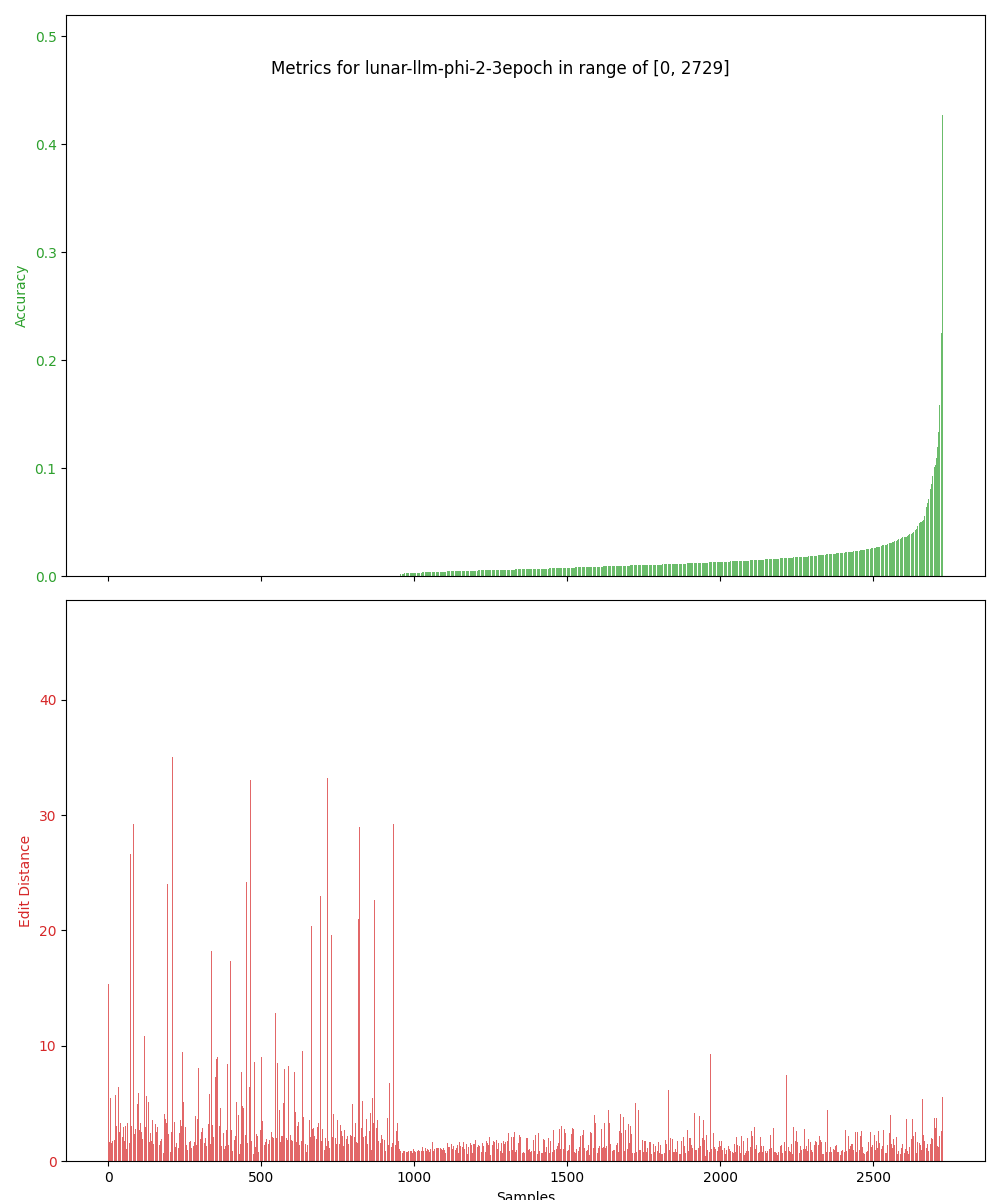
\includegraphics[width=1.0\textwidth]{Immagini/evaluations/lunar-llm-phi-2-3epoch_metrics.png}
	\end{subfigure}%
	\begin{subfigure}{0.5\textwidth}
		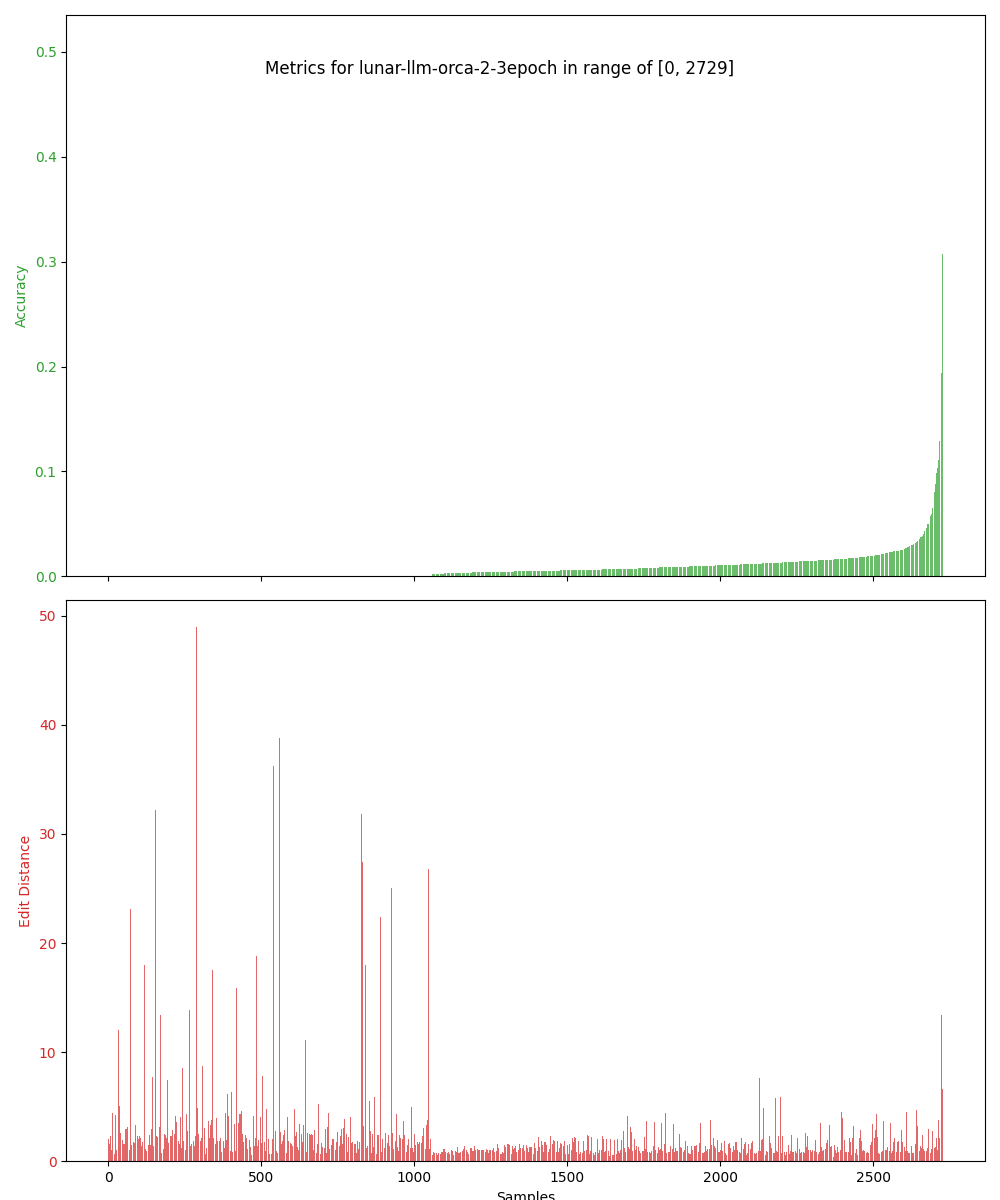
\includegraphics[width=1.0\textwidth]{Immagini/evaluations/lunar-llm-orca-2-3epoch_metrics.png}
	\end{subfigure}
 	\begin{subfigure}{0.5\textwidth}
		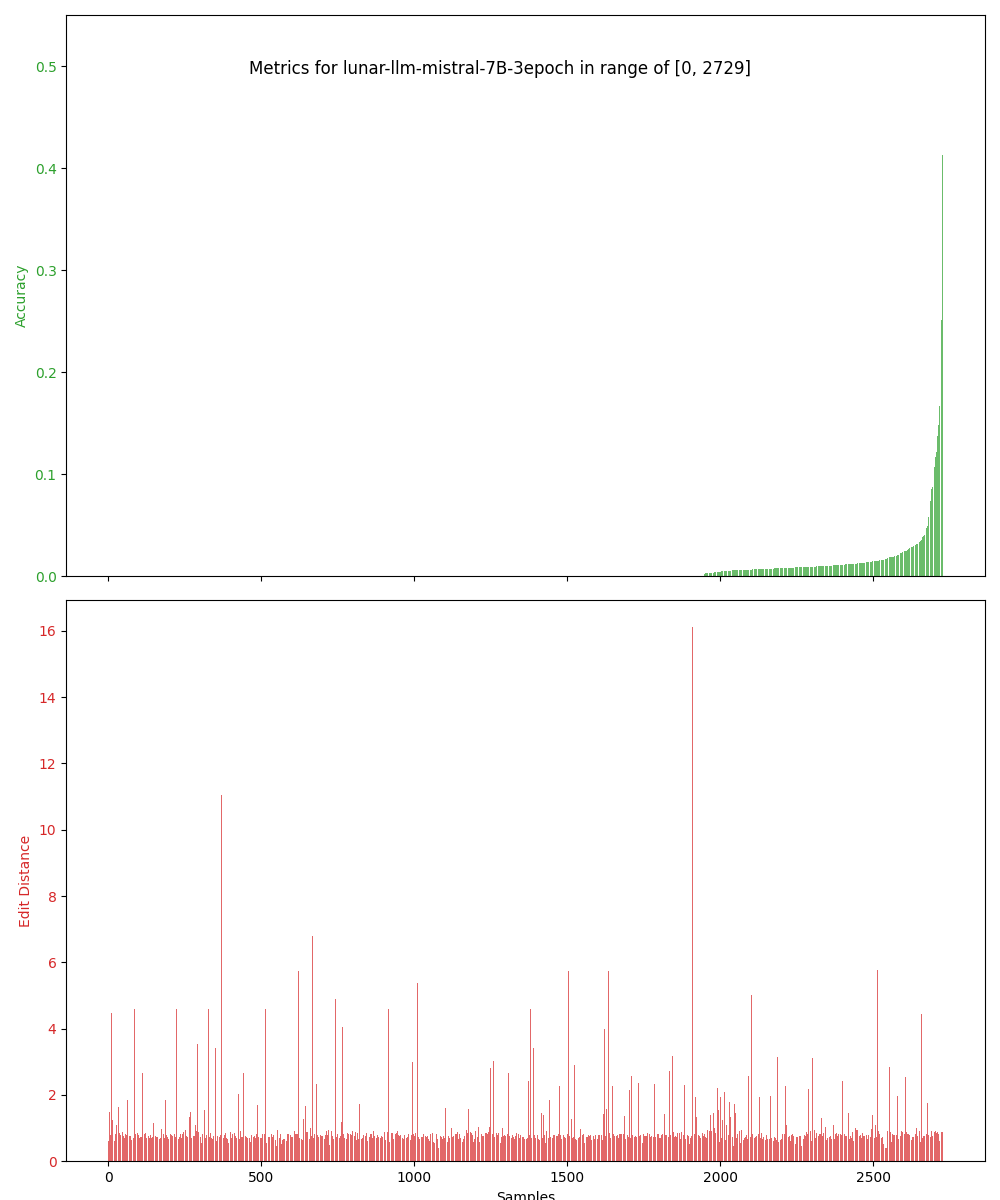
\includegraphics[width=1.0\textwidth]{Immagini/evaluations/lunar-llm-mistral-7B-3epoch_metrics.png}
	\end{subfigure}%
 	\begin{subfigure}{0.5\textwidth}
		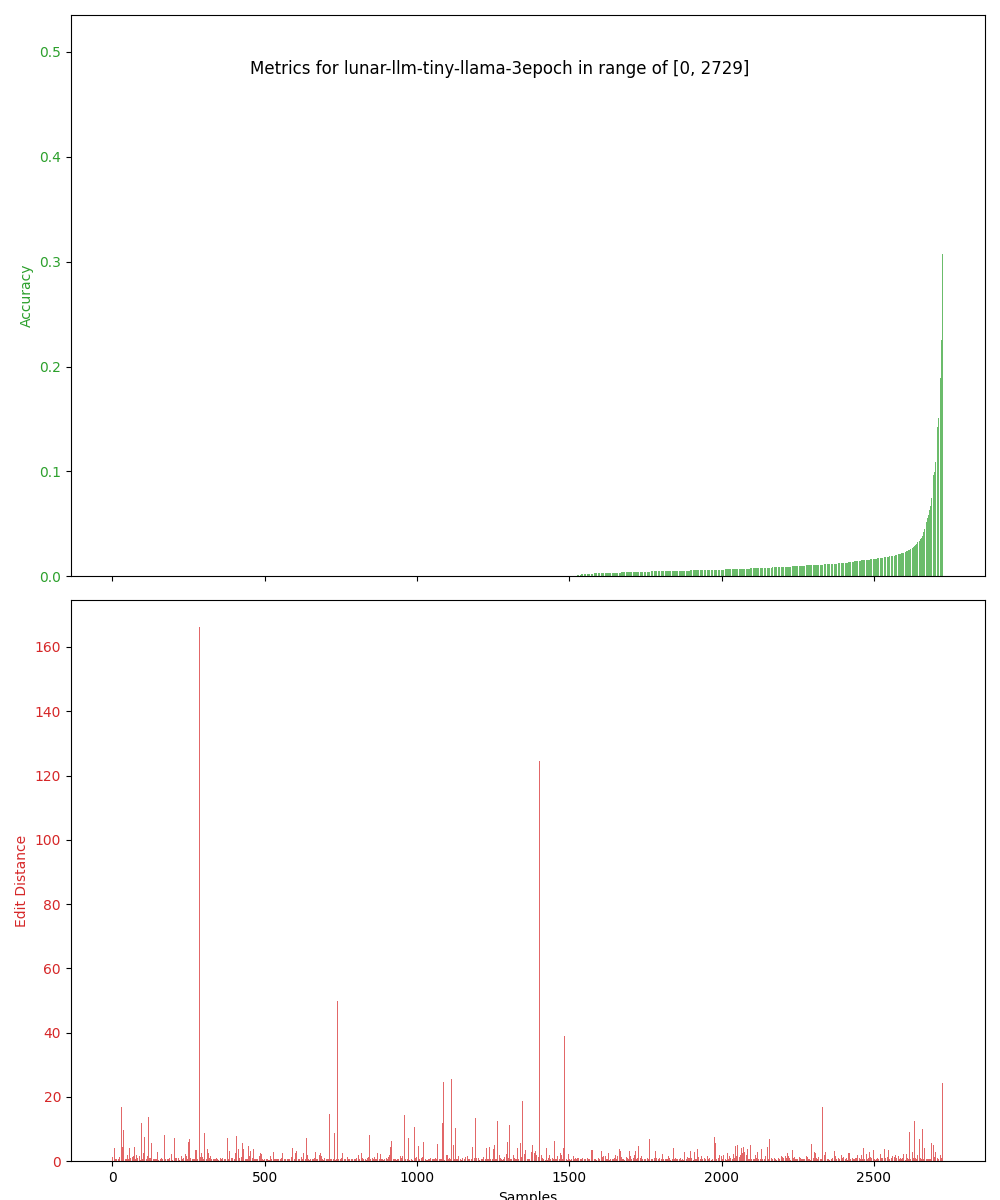
\includegraphics[width=1.0\textwidth]{Immagini/evaluations/lunar-llm-tiny-llama-3epoch_metrics.png}
	\end{subfigure}
	\caption{Andamenti di Edit Distance e Accuratezza per LLM}
	\label{fig:llm_metrics}
\end{figure}

\begin{table}[ht]
	\centering
	\resizebox{0.99\linewidth}{!}{
		\begin{tabular}{||c||c|c|c|c||}
			\hhline{|t:=:t:+====:t|}
			LLM &\phantom{00}Organizzazione\phantom{00}&\phantom{00}Parametri\phantom{00}&\phantom{00}Media Perplexity\phantom{00}&\phantom{00}Varianza Perplexity\phantom{00} \\
			\hhline{|:=::====:|}
               \href{https://huggingface.co/mistralai/Mistral-7B-v0.1}{Mistral}&Mistral AI&7 Miliardi & 460,562510 & $2,910612\cdot10^5$   \\
			\hhline{||-||----||}
            \href{https://huggingface.co/microsoft/Orca-2-13b}{Orca 2}&Microsoft&13 Miliardi&205,080949& $1,639549\cdot10^5$ \\
			\hhline{||-||----||}
            \href{https://huggingface.co/microsoft/phi-2}{Phi-2}&Microsoft&2.7 Miliardi& 208,279878 & $2,069949\cdot10^4$ \\
			\hhline{||-||----||}
            \href{https://huggingface.co/TinyLlama/TinyLlama-1.1B-Chat-v1.0}{TinyLlama}&TinyLlama&1.1 Miliardi &12494,401646& $8,721912\cdot10^8$  \\
			\hhline{||-||----||}
            \hhline{|b:=:b:+====:b|}
		\end{tabular}
	}
	\vspace*{2mm}
	\caption{Media e varianza di Perplexity per ogni LLM}
	\label{tab:llm_perplexity}
\end{table}

\subsection{Test qualitativo}\label{sec:hpc_unipr_inference}


In questa sotto sezione, viene descritto il test qualitativo condotto per valutare i modelli di linguaggio addestrati, considerando diversi aspetti rilevanti per un'azienda che desidera investire nello sviluppo del proprio GCC investendo nel campo dell'intelligenza artificiale per la generazione degli script delle carte. 

Gli aspetti presi in considerazione sono:

\begin{enumerate}[label=\alph*.]
    \item Numero di epoche necessarie per raggiungere un risultato accettabile, da cui ne deriva il relativo costo energetico per l'affitto di una GPU per l'addestramento.
    \item Dimensione del modello, tenendo conto dell'hosting dell'inferenza su una macchina virtuale nel cloud.
    \item Tempo di risposta del modello dato l'input in esame.
    \item Qualità e verosimiglianza dell'output generato rispetto al risultato atteso.
\end{enumerate}

Il test è stato effettuato caricando l'inferenza del modello e richiedendo ai vari modelli di generare lo script di diverse carte dell'ultima espansione di \emph{Magic}, quindi carte mai viste dal modello durante l'addestramento. Per confrontare qualitativamente i diversi LLM, si fa riferimento alla tabella \ref{tab:llm_inference}. Il codice utilizzato per effettuare il test è mostrato nel Codice \ref{lst:inference}, mentre un esempio di output ottenuto è presentato nel Codice \ref{lst:inference_output}.

Analizzando i risultati ottenuti, è possibile valutare le prestazioni dei vari modelli in termini di epoche necessarie per raggiungere un risultato accettabile, costo energetico per l'affitto di una GPU, dimensione del modello e tempo di risposta. Inoltre, confrontando gli output generati, è possibile identificare il modello che produce risultati qualitativamente migliori e più verosimili rispetto a quelli attesi. Questa analisi consente di prendere decisioni informate sull'investimento nel GCC digitale e sulla scelta del modello più adatto alle esigenze dell'azienda.


\begin{table}[ht]
	\centering
	\resizebox{0.99\linewidth}{!}{
		\begin{tabular}{||c||c|c|c|c|c|c||}
			\hhline{|t:=:t:+======:t|}
			LLM &\phantom{00}Organizzazione\phantom{00}&\phantom{00}Parametri\phantom{00}&\phantom{00}Epoche\phantom{00}&\phantom{00}Risultato qualitativo\phantom{00}&\phantom{00}Tempo di risposta (hh:mm:ss)\phantom{00}&\phantom{00}Dimensione (GB)\phantom{00} \\
			\hhline{|:=::======:|}
			\href{https://huggingface.co/teknium/OpenHermes-7B}{OpenHermes}&Teknium&7 miliardi&10&\checkmark& 2:27:59 & 11 \\
			\hhline{||-||------||}
               \href{https://huggingface.co/mistralai/Mistral-7B-v0.1}{Mistral}&Mistral AI&7 Miliardi & 10& \checkmark & 23:32 & 15  \\
			\hhline{||-||------||}
            \href{https://huggingface.co/microsoft/Orca-2-13b}{Orca 2}&Microsoft&13 Miliardi&3&\checkmark & 14:23 & 27 \\
			\hhline{||-||------||}
            \href{https://huggingface.co/microsoft/phi-2}{Phi-2}&Microsoft&2.7 Miliardi& 3 & \checkmark & 5:06 & 5.5\\
			\hhline{||-||------||}
            \href{https://huggingface.co/TinyLlama/TinyLlama-1.1B-Chat-v1.0}{TinyLlama}&TinyLlama&1.1 Miliardi &20& & 9:43 & 2.2   \\
			\hhline{||-||------||}
            \hhline{|b:=:b:+======:b|}
		\end{tabular}
	}
	\vspace*{2mm}
	\caption{LLM a confronto}
	\label{tab:llm_inference}
\end{table}

È importante aggiungere che il test qualitativo è stato effettuato anche su alcuni LLM senza fine tuning, come ChatGPT 3.5 e 4. Tuttavia, il risultato del test per questi modelli è stato insoddisfacente, poiché il prompt è stato semplicemente rielaborato, senza generare lo script di una carta come richiesto. Questo evidenzia l'importanza del fine tuning per ottenere risultati migliori e più accurati in base alle specifiche esigenze del dominio applicativo.

\begin{algorithm}[ht]
	\caption{Script di inferenza di un LLM}
	\label{lst:inference}
	\begin{Verbatim}[numbers=left,breaklines]
def run_inference(model, tokenizer, prompt, max_length=300):
    # Encode the prompt text
    input_ids = tokenizer.encode(prompt, return_tensors='pt')
    
    # Generate text using the model
    output_sequences = model.generate(
        input_ids=input_ids,
        max_length=max_length,
        temperature=0.5,
        top_k=50,
        top_p=0.95,
        pad_token_id=tokenizer.eos_token_id,
        do_sample=True
    )
    
    # Decode the generated text
    generated_text = tokenizer.decode(output_sequences[0], skip_special_tokens=True)
    
    return generated_text
	\end{Verbatim}
\end{algorithm}

\begin{algorithm}[ht]
	\caption{Esempio di output ottenuto da microsoft/phi-2 }
	\label{lst:inference_output}
        \footnotesize
	\begin{Verbatim}[numbers=left,breaklines]
### Question: Create the Forge script for this magic card
{
    "name": "Wrench",
    "mana_cost": "{W}",
    "type_line": "Artifact— Clue Equipment", 
    "oracle_text":  "Equipped creature gets +1/+1 and has vigilance and \"{3}, {T}: Tap target creature.\"\n{2}, Sacrifice CARD_NAME: Draw a card.\nEquip {2}"
} 
### Response: 
Name:Wrench
ManaCost:W
Types portfolios:Artifact—Clue Equipment
S:Mode$ Continuous | Affected$ Creature.EquippedBy | AddPower$ 1 | AddToughness$ 1 | AddKeyword$ Vigilance | AddAbility$ Tap | Description$ Equipped creature gets +1/+1 and has vigilance and "{3}, {T}: Tap target creature."
SVar:Tap:AB$ Tap | Cost$ 3 T | ValidTgts$ Creature | TgtPrompt$ Select target creature | SpellDescription$ Tap target creature.
A:AB$ Draw | Cost$ 2 Sac<1/CARDNAME> | NumCards$ 1 | SpellDescription$ Draw a card.\nK:Equip:2
Oracle:Equipped creature gets +1/+1 and has vigilance and "{3}, {T}: Tap target creature."\n{2}, Sacrifice Wrench: Draw a card\nEquip {2}
### Expected:
Name:Wrench
ManaCost:W
Types:Artifact Clue Equipment
S:Mode$ Continuous | Affected$ Creature.EquippedBy | AddAbility$ ABTap | AddPower$ 1 | AddToughness$ 1 | AddKeyword$ Vigilance | Description$ Equipped creature gets +1/+1 and has vigilance and "{3}, {T}: Tap target creature."
SVar:ABTap:AB$ Tap | Cost$ 3 T | ValidTgts$ Creature | SpellDescription$ Tap target creature.
A:AB$ Draw | Cost$ 2 Sac<1/CARDNAME> | NumCards$ 1 | SpellDescription$ Draw a card.
K:Equip:2
DeckHas:Ability$Sacrifice
Oracle:Equipped creature gets +1/+1 and has vigilance and "{3}, {T}: Tap target creature."\n{2}, Sacrifice Wrench: Draw a card.\nEquip {2}
	\end{Verbatim}
\end{algorithm}

